\label{sec:H2OF}
\subsection{Standard Theory}
\label{subsec:stdH2OF}
We now consider a discrete-time, linear, time-invariant system, $P$, of the form $$P \shorteq \arr{c}{\hspace{0.8cm}\stackrel{n}{\leftrightarrow}\hspace{0.5cm}\stackrel{l}{\leftrightarrow}\hspace{0.6cm}\stackrel{m}{\leftrightarrow} \\\arr{c}{\scriptstyle{n} \,\updownarrow\\\scriptstyle{p} \,\updownarrow\\\scriptstyle{q} \,\updownarrow} \ma{\arr{c|cc}{ A&B_1&B_2\\\hline C_1&D_{11}&D_{12}\\C_2&D_{21}&0}}},$$
which satisfies (A1)-(A3) as well as:
\begin{itemize}
\item[(A4)] $(A,C_2)$ is detectable 
\item[(A5)] $D_{21}D_{21}'>0$
\item[(A6)] rank$\ma{A-e^{j\theta}I&B_1\\C_2& D_{21}}=n+q\quad \forall\, \theta \,\in (-\pi,\pi]$.
\end{itemize}
%
We wish to compute an internally stabilising $K$ that minimises $\nrm{F_l(P,K)}_2$. Define:
\als{
    \bar S&=D_{21}D_{21}'+C_2YC_2' &  L_2&=-(AYC_2'+B_1D_{21}')\bar S^{-1}
}
%
If $(A4)$-$(A6)$ are satisfied, it is shown in \cite{ZDG} that there exists a $Y$ that solves
\aln{
Y=AYA'-L_2 {\bar S}L_2'+B_1B_1'
\label{eqn:Y2d}
}
such that 
\als{
Y\geq 0\\
A+L_2C_2 &\textrm{ is asymptotically stable}.
}
If we define: 
\als{
L_0=(F_2YC_2'+F_0D_{21}'){\bar S}^{-1},
}
then, according to \cite{ZDG}, the $\htwo$-optimal output feedback controller is given by:
\aln{
K& \shorteq \ma{\arr{c|c}{A_K&B_K\\ \hline C_K &D_K}} \label{eqn:H2OptK}\\ 
A_K&=A+B_2F_2+L_2C_2-B_2L_0C_2\\
B_K&=-(L_2-B_2L_0)\\
C_K&=F_2-L_0C_2\\
D_K&=L_0.}

The $\htwo$-norm of the resulting closed loop system is given by:
\mls{\nrm{F_l(P,K)}_2^2=\nrm{F_l(P_{FI},K_{FI})}_2^2\\
	+\tra{\bar R\right( (L_0D_{21}-F_0)(L_0D_{21}-F_0)' +(L_0C_2-F_2)Y(L_0C_2-F_2)'\left) }}


\subsection{Efficient computation of Output Feedback controller}
In this section we aim to find a computationally efficient solution to the DARE (\ref{eqn:Y2d}), given that P has the structure described in (\ref{eqn:P}). The results of this section do not depend on the internal structure of $A_p$, $B_p$ and $C_p$ (though we do require that $A_p$ is stable).

\begin{lem} 
The stabilising non-negative solution to (\ref{eqn:Y2d}) may be computed using:
\als{
Y&=
	\arr{r}{
	\stackrel{n_g}{\leftrightarrow}\hspace{0.2cm}
	\stackrel{Nl_r+n_r}{\leftrightarrow}\hspace{0cm}\\
	%%
	\arr{r}{
	\scriptstyle{n_g} \,\updownarrow\\
	\scriptstyle{Nl_r+n_r} \,\updownarrow}
	\ma{\arr{cc}{ Y_{g} & \hspace{0.2cm}0 \\ 0&\hspace{0.2cm}0}}
	}
,}
where $Y_g$ is the unique stabilising and non-negative solution to:
\aln{
Y_g&=A_gY_gA_g'-L_{2g} {\bar S_g}L_{2g}'+B_{1gw}'B_{1gw} \label{eqn:Y2g}}
with
\als{
\bar S_g&=D_{21gw}D_{21gw}'+C_{2g}Y_gC_{2g}' &  
	L_{2g}&=-(A_gY_gC_{2g}'+B_{1gw}D_{21gw}')\bar S_g^{-1}\nonumber.
}
\end{lem}
\begin{pf}
Note that $(A4)-(A6)$ imply 
\begin{itemize}
\item[(A4g)] $(A_g,C_{2g})$ is detectable; 
\item[(A5g)] $D_{21gw}D_{21gw}'>0$;
\item[(A6g)] rank$\ma{A_g-e^{j\theta}I&B_{1gw}\\C_{2g}& D_{21gw}}=n_g+q_g\quad \forall\, \theta \,\in (-\pi,\pi]$.
\end{itemize}
%
It then follows that $(A4)-(A6)$ ensure the existence of a stabilising nonnegative solution to (\ref{eqn:Y2g}). 
Let $Y_g$ be a stabilising and non-negative solution to (\ref{eqn:Y2g}). We will now show that $Y=\ma{Y_g&0\\0&0}$ is a stabilising nonnegative solution to (\ref{eqn:Y2d}).

It easily checked that the following hold if $Y=\ma{Y_g&0\\0&0}$:
\aln{
\bar S&=\ma{\bar S_g & 0\\0& D_rD_r'}\nonumber\\
L_2&=\ma{L_{2g} &0\\0& -B_dD_r^{-1}}\label{eqn:L2struct}\\
B_1B_1'&=\ma{ B_{1gw}B_{1gw}' & 0\\0& B_dB_d'}\nonumber\\
AYA'&= \ma{A_gY_gA_g'  &0 \\0 &0}\nonumber
,}
where the invertibility of $D_r$ is guaranteed by assumption $(A5)$, together with the fact that $W_r$ is square. It then follows that:
\als{
\spl{AYA'-L_2 {\bar S}\bar L_2'+B_1B_1'&=\ma{A_gY_gA_g'-L_{2g} {\bar S_g}\bar L_{2g}'+B_{1gw}B_{1gw}'&0\\0&0}}\\
&=\ma{Y_g&0\\0&0}=Y.
}
Therefore, if $Y_g$ solves (\ref{eqn:Y2g}), then $Y=\ma{Y_g&0\\0&0}$ solves (\ref{eqn:Y2d}). We now need to check that $Y$ is stabilising. Note that:
\als{
&A+L_2C_2=\ma{A_g+L_{2g}C_{2g}&\star\\0&A_d-B_dD_r^{-1}C_{d2}}.
}
The matrix $A_d-B_dD_r^{-1}C_{d2}$ is stable because:
\aln{
A_d-B_dD_r^{-1}C_{d2}&=\ma{A_p&0\\0&A_r-B_rD_r^{-1}C_r}\label{eqn:AdBdDrCd2},
}
in which $A_p$ is stable by definition and $A_r-B_rD_r^{-1}C_r$ is stable because $W_r$ is assumed to be outer. Since $Y_g$ is stabilising, we know that $A_g+L_{2g}C_{2g}$ is stable, and hence that $A+L_2C_2$ is stable, as required. 
 \end{pf}

\subsection{Efficient implementation}
\label{sec:EffImp}
We now have a complete method for efficiently computing the output feedback preview controller, however, in its present form, this controller has the same order as the generalized plant. In general, a controller of this order cannot be implemented. Fortunately the high-order part of the controller is an FIR filter (illustrated in Figure \ref{fig:PrevContStruct}), for which efficient implementations exist.
{
\stdcontrolfrags
\psfrag{Order ng}{Order $n_g$}
\psfrag{Order nr}{Order $n_r$}
\psfrag{Order Nlr}{Order $Nl_r$}
\psfrag{FIR}{FIR}
\psfrag{IIR}{IIR}
\begin{figure}
\begin{center}
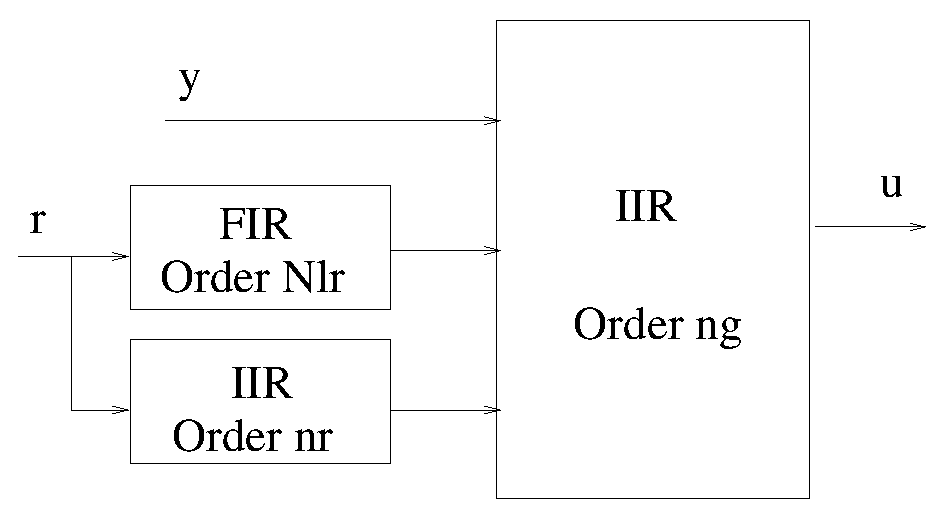
\includegraphics[width=8cm]{./diags/PrevContStruct.eps}
\caption{\label{fig:PrevContStruct} Structure of the $\htwo$-optimal preview controller. The signal $u$ is the control, the measurement is $y$, and $r$ is the future value of the previewable disturbance. The preview length is $N$, $l_r$ is the dimension of $r$, $n_r$ is the order of $W_r$ and $n_g$ is the order of $G$. }
\end{center}
\end{figure}
}


This controller structure is proved in the following Lemma:
%, which just requires the shifting of a block of memory. 


\begin{lem}
The optimal controller described in (\ref{eqn:H2OptK}) for the plant in (\ref{eqn:P}) can be written in the form: 
\aln{
K \shorteq \ma{\arr{c|c}{A_K&B_K\\ \hline C_K &D_K}}
=\ma{\arr{ccc|cc}{A_{Kgg} &A_{Kgp} & A_{Kgr} & B_{Kgy}& B_{Kgr}\\
                  0&A_p&0&0&B_p\\
                  0&0&A_r-B_rD_r^{-1}C_r &0 &B_rD_r^{-1}\\\hline
                  C_{Kg}& C_{Kp}& C_{Kr}& L_{0y}&F_{0r}D_{r}^{-1}}}\label{eqn:StructController}}
where $\szo{A_{Kgg}}{n_g\times n_g}$ and $\szo{B_{Kgg}}{n_g\times l_w}$ and
\als{
L_{0y}&=(F_{2g}Y_gC_{2g}'+F_{0w}D_{21gw}'){\bar S_g}^{-1}\\
A_{Kgg}&=A_g+B_{2g}F_{2g}+L_{2g}C_{2g}-B_{2g}L_{0y}C_{2g} \\
A_{Kgp}&=B_{1gr}C_p+B_{2g}F_{2p}+L_{2g}D_{21gr}C_p-B_{2g}L_{0y}D_{21gr}C_p\\
A_{Kgr}&=B_{2g}F_{2r}-B_{2g}F_{0r}D_r^{-1}C_r\\
B_{Kgy}&=-(L_{2g}-B_{2g}L_{0g})\\
B_{Kgr}&=B_{2g}F_{0r}D_r^{-1}\\
C_{Kg}&=F_{2g}-L_{0y}C_{2g}\\
C_{Kp}&=F_{2p}-L_{0y}D_{21gr}C_p\\
C_{Kr}&=F_{2r}-F_{0r}D_r^{-1}C_r
}
\end{lem}
\begin{pf} The realization given in (\ref{eqn:StructController}) follows from (\ref{eqn:H2OptK}), together with (\ref{eqn:L2struct}),  (\ref{eqn:AdBdDrCd2}) and:
\als{L_0=\ma{L_{0y} & F_{0r}D_r^{-1}}.}
\end{pf}
%
This then leads to the low-order implementation:
\begin{equation}
\bar K \shorteq \ma{\arr{cc|ccc}{A_{Kgg}  & A_{Kgr} & B_{Kgy}& A_{Kgp} &B_{Kgr}\\
                  0&A_r-B_rD_r^{-1}C_r &0 &0&B_rD_r^{-1}\\\hline
                  C_{Kg}&  C_{Kr}& L_{0y}&C_{Kp}&F_{0r}D_{r}^{-1}}}, \label{low_order_K}
\end{equation}
where that the optimal control is given by
\als{
u^*&=\bar K \ma{y\\\bar r}\\
\bar r(k)&=\ma{r(k-N)\\\vdots\\r(k)}.
}

\begin{cor}
\label{cor:minwandr}
The output feedback controller that minimises $\nrm{T_{v\rightarrow z}}_2$, also minimises $\nrm{T_{\eta\rightarrow z}}_2$ and $\nrm{T_{w\rightarrow z}}_2$.
\end{cor}
\begin{pf}
The controller may be decomposed into feedback and feedforward components $K_{fb}$ and $K_{ff}$, so that 
\als{u^*=K_{fb}y+K_{ff}r,} 
with $K_{fb}$ given by:
\als{
K_{fb}\shorteq \ma{\arr{c|c}{A_{Kgg}&B_{Kgy}\\ \hline C_{Kg} &L_{0y}}}
.}

The transfer function $T_{w\rightarrow z}$ is determined by $K_{fb}$ and $P$, and it is  easily checked that $K_{fb}$ is precisely the controller which is obtained by minimising $\nrm{T_{w\rightarrow z}}_2$ alone.

It is well known that the $\htwo$-optimal controller has an observer structure. If $w=0$, then the observer will contain an exact copy of the states of $G$ and $W_r$ (once intial transients have decayed). Therefore the closed-loop transfer function $T_{r\rightarrow z}$ will be precisely the same as that resulting from application of the full information controller, $K_{FI}$ to the plant $P_{FI}$. Remark~\ref{rem:FIminwandr} implies that the value of $\nrm{T_{r\rightarrow z}}_2$ achieved by the this controller is indeed minimal.
\end{pf}

Unlike the full information case, this result is not a general property of any partition of the exogenous disturbance signal, instead it results from the particular structure considered here. The result is useful because it leads us to the conclusion that the choice of $W_r$ does not alter the resulting  $T_{w\rightarrow z}$, and so $W_r$ tunes only the response to the previewable signal. 









